\documentclass[11pt]{article}
\usepackage{geometry,marginnote} % Pour passer au format A4
\geometry{hmargin=1cm, vmargin=1cm} % 

% Page et encodage
\usepackage[T1]{fontenc} % Use 8-bit encoding that has 256 glyphs
\usepackage[english,french]{babel} % Français et anglais
\usepackage[utf8]{inputenc} 

\usepackage{lmodern,numprint}
\setlength\parindent{0pt}

% Graphiques
\usepackage{graphicx,float,grffile,units}
\usepackage{tikz,pst-eucl,pst-plot,pstricks,pst-node,pstricks-add,pst-fun} 

% Maths et divers
\usepackage{amsmath,amsfonts,amssymb,amsthm,verbatim}
\usepackage{multicol,enumitem,url,eurosym,gensymb,tabularx}

\DeclareUnicodeCharacter{20AC}{\euro}



% Sections
\usepackage{sectsty} % Allows customizing section commands
\allsectionsfont{\centering \normalfont\scshape}

% Tête et pied de page
\usepackage{fancyhdr} \pagestyle{fancyplain} \fancyhead{} \fancyfoot{}

\renewcommand{\headrulewidth}{0pt} % Remove header underlines
\renewcommand{\footrulewidth}{0pt} % Remove footer underlines

\newcommand{\horrule}[1]{\rule{\linewidth}{#1}} % Create horizontal rule command with 1 argument of height

\newcommand{\Pointilles}[1][3]{%
  \multido{}{#1}{\makebox[\linewidth]{\dotfill}\\[\parskip]
}}

\newtheorem{Definition}{Définition}

\usepackage{siunitx}
\sisetup{
    detect-all,
    output-decimal-marker={,},
    group-minimum-digits = 3,
    group-separator={~},
    number-unit-separator={~},
    inter-unit-product={~}
}

\setlength{\columnseprule}{1pt}

\begin{document}

\setlength{\columnseprule}{0pt}

\horrule{2px}
\section*{Chapitre 6 - Calcul littéral}
\horrule{2px}

\section*{Les petits problèmes}

\begin{multicols}{2}

  On a réparti 5,4kg de confiture de cerises dans 19 pots de 3 tailles différentes. Sur chaque étagères, il  y a exactement le même poids de confiture. \\
  Quelle quantité de confiture chaque pot contient-il ?
  
  \begin{figure}[H]
    \centering
    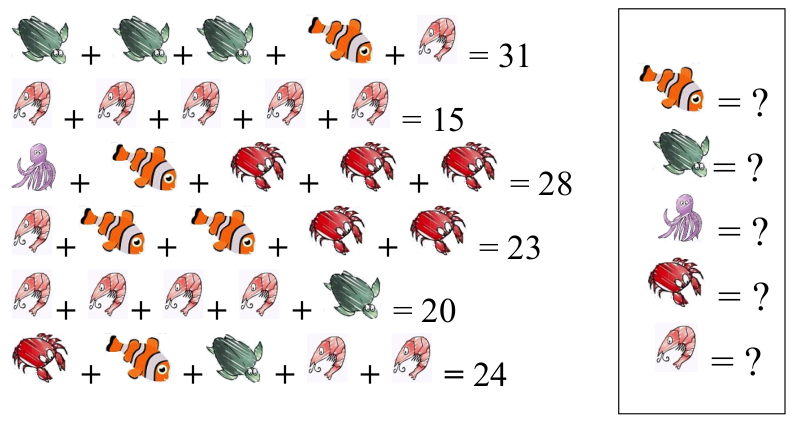
\includegraphics[width=0.8\linewidth]{5x6-calcul-litteral/poissons-1.png}
  \end{figure}

  \begin{figure}[H]
    \centering
    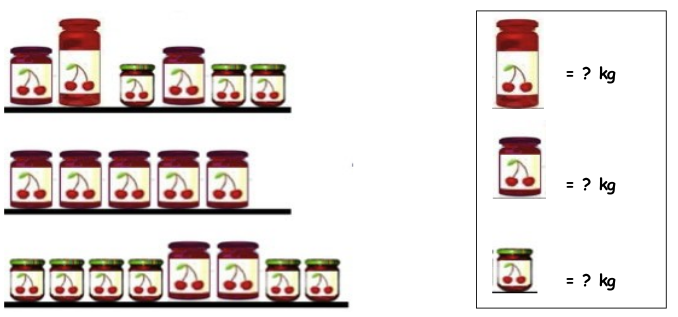
\includegraphics[width=0.8\linewidth]{5x6-calcul-litteral/confitures.png}
  \end{figure}

  \begin{figure}[H]
    \centering
    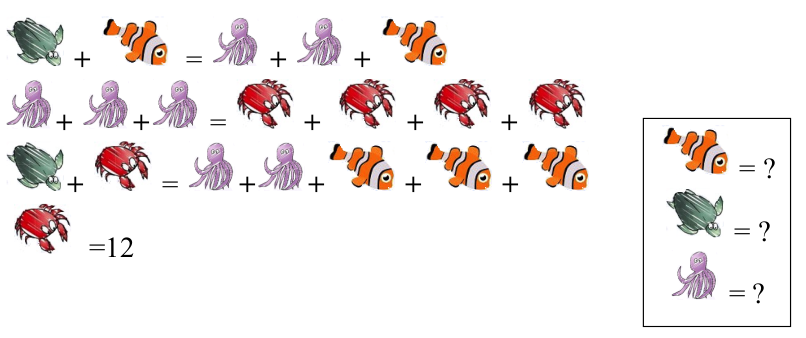
\includegraphics[width=0.8\linewidth]{5x6-calcul-litteral/poissons-2.png}
  \end{figure}

\end{multicols}

On ne cherche pas à un résultat mais un nombre dans un calcul. Le signe = ne signifie pas seulement \textit{\og la réponse est \fg}. Le signe égal signale un équilibre, une égalité qui peut être lue dans les deux sens.

\begin{Definition}{Sens du signe =}\\
  Ce qui est à gauche = Ce qui est droite. 
\end{Definition}

\textbf{Exercice :} \\

\begin{flalign*}
  \triangle &= 12 \\
  \triangle + 1 &= 13 \\
  \triangle + 2 &= 14 \\
  \triangle - 1 &= 11 \\
  \triangle + \triangle &= 24 \\
  4 \times \triangle &= 48
\end{flalign*}

En mathématiques, on ne va faire de petits dessins sur sa copie. On va utiliser une lettre pour ça : $x$. \\

  \textbf{Exercice type 1 : Calculer} \\
  On pose $x = 10$ et $a = 2,5$. 

  \begin{itemize}[label={$\bullet$}]
    \item $x + 2 = 12 $
    \item $x + a = 12,5 $
    \item $10 \times a + 4 \times b = 65$
    \item $\dfrac{x}{a} + 1 = 5 $
  \end{itemize}

\newpage

\section*{Le Petit Prince}

\begin{multicols}{2}

  \begin{figure}[H]
    \centering
    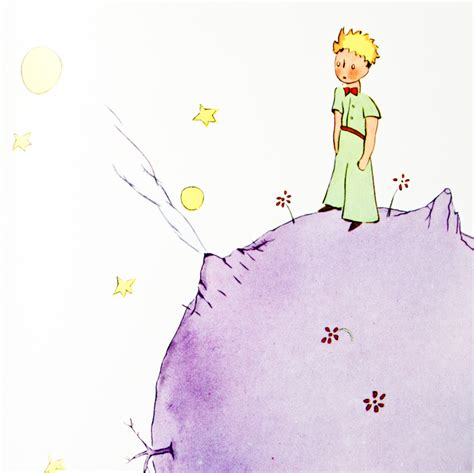
\includegraphics[width=0.8\linewidth]{5x6-calcul-litteral/pp.png}
  \end{figure}

\subsection*{En savoir plus}

\begin{itemize}
\item Wikipedia : \url{https://fr.wikipedia.org/wiki/Le_Petit_Prince}
\item Wikipedia : \url{https://fr.wikipedia.org/wiki/Antoine_de_Saint-Exup%C3%A9ry}
\item Site officiel : \url{https://www.lepetitprince.com/}
\end{itemize}


On suit un aviateur qui tombe en panne et se pose en catastrophe dans le désert du Sahara. Il n’arrive pas à réparer son avion. Le lendemain, il est réveillé par un petit personnage qui lui demande: \og S'il vous plaît… dessine-moi un mouton! \fg 

\end{multicols}

\textit{(Extrait du Petit Prince...)}

\begin{multicols}{2}
  \og S'il vous plaît… dessine-moi un mouton ! \fg\\
  Alors j'ai dessiné.
  
  \begin{figure}[H]
    \centering
    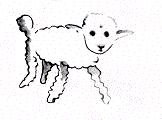
\includegraphics[width=0.3\linewidth]{5x6-calcul-litteral/mouton2.png}
  \end{figure}

  Il regarda attentivement, puis: \\
  - Non! Celui-là est déjà très malade. Fais-en un autre. \\
  Je dessinai:

  \begin{figure}[H]
    \centering
    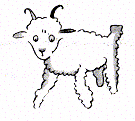
\includegraphics[width=0.3\linewidth]{5x6-calcul-litteral/mouton1.png}
  \end{figure}

  Mon ami sourit gentiment, avec indulgence: \\
  - Tu vois bien... ce n'est pas un mouton, c'est un bélier. Il a des cornes... \\
  Je refis donc encore mon dessin:

  \begin{figure}[H]
    \centering
    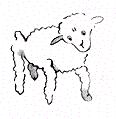
\includegraphics[width=0.3\linewidth]{5x6-calcul-litteral/mouton3.png}
  \end{figure}
  
  Mais il fut refusé, comme les précédents: \\
  - Celui-là est trop vieux. Je veux un mouton qui vive longtemps. \\
  Alors, faute de patience, comme j'avais hâte de commencer le démontage de mon moteur, je griffonnai ce dessin-ci.
  
  \begin{figure}[H]
    \centering
    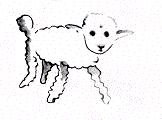
\includegraphics[width=0.3\linewidth]{5x6-calcul-litteral/mouton2.png}
  \end{figure}

  Et je lançai: \\
  - Ça c'est la caisse. Le mouton que tu veux est dedans. \\
  Mais je fus bien surpris de voir s'illuminer le visage de mon jeune juge: \\
  - \textbf{C'est tout à fait comme ça que je le voulais ! }
\end{multicols}

Comme l'aviateur, on va utiliser \textbf{une boite à nombre : } $x$. Dedans on va mettre le nombre qui répond à la question. Ce n'est pas un nombre au hasard. Ce nombre est une solution de notre problème. Il n'est pas (encore) connu.

\begin{Definition}{La boite à nombre : $x$}\\
  Le nombre $x$ est inconnu et solution. 
\end{Definition}

\newpage 

\section*{Factoriser}

En mathématiques, quand on utilise des nouveaux nombres, on a besoin \textbf{d'adapter} less opérations. Ici, le nombre $x$ étant inconnu, on ne va pas pouvoir donner de résultat. Par contre, on va pouvoir \textbf{réduire}. 

\begin{flalign*}
  5 \times 3 &= 3 + 3 + 3 + 3 + 3 \\
  5 \times x &= x + x + x + x + x 
\end{flalign*}

La multiplication est une répétition. 

\begin{flalign*}
  3 \times x + x  &= x + x + x + x  = 4 \times x \\
  3 \times x - x  &= x + x + x - x  = 2 \times x \\
  3 \times x + 1  &= x + x + x + 1  = 3 \times x + 1 
\end{flalign*}

\textbf{Remarques} : 

\begin{itemize}[label={$\bullet$}]
  \item $6 \times x = x \times 6 = 6x$
  \item $1 \times x = 1x = x$
  \item $0 \times x = 0$
\end{itemize}

\textbf{Exercice type 2 : Représenter les $\times$ en $+$} 

\begin{itemize}[label={$\bullet$}]
  \item $3 \times x = x + x + x$
  \item $4x = x + x + x + x$
  \item $2x + x \times 3 = x + x + x + x + x $
  \item $4x + 6 = x + x + x + x + 6$
\end{itemize}

\textbf{Exercice type 3 : Réduire} 

\begin{itemize}[label={$\bullet$}]
  \item $3 \times x = 3x$
  \item $40x + 60x = 100x$
  \item $12x - x = 11 x $
  \item $4 \times x + 6 = 4x + 6$
\end{itemize}

\section*{Mise en équation}



\section*{Équations}



\newpage 

\section*{Annexe}

\textbf{Le Petit Prince} est un court roman très connu écrit par Antoine de Saint-Exupéry. 
C'est une œuvre poétique et philosophique qui prend l'apparence d'un conte pour enfants. 

\begin{center}
  {\fontfamily{jkplos}\selectfont \og On ne voit bien qu'avec le cœur. L'essentiel est invisible pour les yeux. \fg }\\
  {\fontfamily{jkplos}\selectfont \og C'est le temps que tu as perdu pour ta rose qui fait ta rose si importante. \fg}\\

\end{center}

\subsection*{l’auteur}
\textbf{Antoine de Saint-Exupéry} est né le 29 juin 1900 à Lyon. Il était  écrivain, poète, aviateur et reporter français. Il est mort le 31 juillet 1944. Il était pilote dans l’armée lorsqu’il a disparu en vol au large de Marseille. Il avait refusé la collaboration.

\subsection*{Poèmes}

{\fontfamily{jkplos}\selectfont 

  \subsubsection*{Aviation}

  \begin{verse}
    Les ailes frémissaient sous le souffle du soir \\
	  Le moteur de son chant berçait l'âme endormie \\
	  Le soleil nous frôlait de sa couleur pâle.
  \end{verse}
  
  \subsubsection*{Guerre}
  
  \begin{verse}
	  Parfois confusément sous un rayon lunaire,\\
	  Un soldat se détache incliné sur l'eau claire ; \\
	  il rêve à son amour, il rêve à ses vingt ans !
  \end{verse}
}


\end{document}
